\documentclass{standalone}

\usepackage{amsmath,amsthm,amsfonts,amssymb}

\usepackage{tikz}
\usetikzlibrary{positioning}

\tikzset{
    node/.style = {
       shape=rectangle, %rounded corners,
       align=center,
       minimum width = .4cm,
       minimum height = .4cm,
 %      fill = gray!30
 %      fill = cyan!40
 %      fill = blue!50!white!80
    },
    Snode/.style = {
       shape=rectangle, %rounded corners,
       align=center,
       minimum width = .4cm,
       minimum height = .4cm,
       fill = green!60!blue!70
    }
%    bad/.style = {
%       shape=rectangle, %rounded corners,
%       align=center,
%       minimum width = .4cm,
%       minimum height = .4cm,
%       fill = red!70
%    }
}
\begin{document}

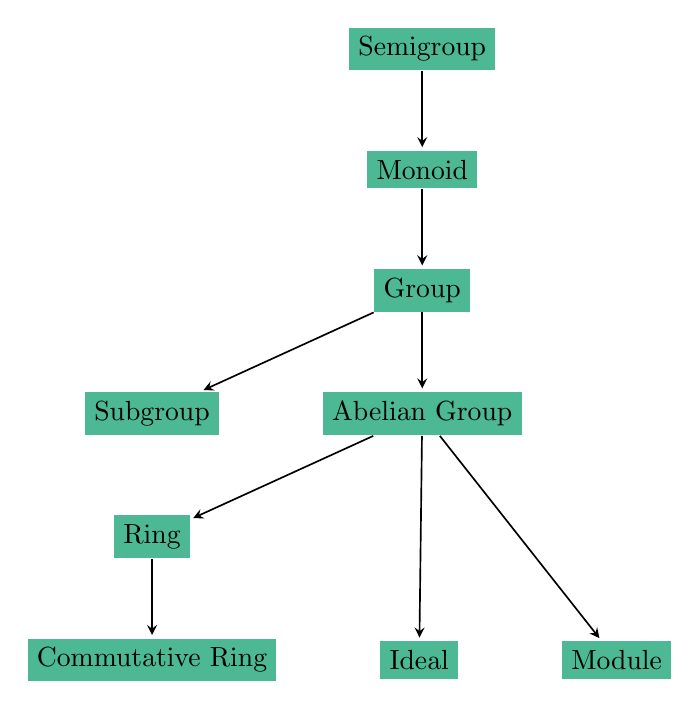
\begin{tikzpicture}[->,>=stealth,shorten >=1pt,auto,node distance=1cm,semithick]
   \node[Snode] (Semigroup) {Semigroup};
   \node[Snode] (Monoid) [below = of Semigroup]{Monoid};
   \node[Snode] (Group) [below =of Monoid] {Group};
   \node[Snode] (AbelianGroup) [below =of Group] {Abelian Group};
   \node[Snode] (Subgroup) [left =1.3cm of AbelianGroup] {Subgroup};
   \node[Snode] (Ring) [below = of Subgroup] {Ring};
   \node[Snode] (CommutativeRing) [below =of Ring] {Commutative Ring};
   \node[Snode] (Ideal) [right =1.3 of CommutativeRing] {Ideal};
   \node[Snode] (Module) [right = 1.3cm of Ideal] {Module};
%   \node[node] (H1) [below = of G1] { };
%   \node[node] (H2) [below = of G2] { };
\path
(Semigroup) edge (Monoid)
(Monoid) edge (Group)
(Group) edge (AbelianGroup)
(Group) edge (Subgroup)
(AbelianGroup) edge (Ideal)
(AbelianGroup) edge (Ring)
(AbelianGroup) edge (Module)
(Ring) edge (CommutativeRing);
%(G1) edge (H1);
%(G2) edge (H2);
\end{tikzpicture}

\end{document}
